\documentclass[11pt,class=article,float=false,crop=false]{standalone}
%\documentclass[11pt]{article}
\usepackage{Part3_packages}

\begin{document}

\section{Résultats et performances}

Dans cette section, nous étudierons dans un premier temps la précision des résultats obtenus, puis nous comparerons les performances des algorithmes. Enfin nous conclurons cette section en proposant un résumé global du comportement des algorithmes proposés en fonction des situations.

\subsection{ Validité des résultats. }

Dans cette section, nous étudierons les conditions de validité des algorithmes proposés. Certains algorithmes peuvent être modifiés afin de trouver un compromis entre performance et précision. Nous étudierons l'impact de la désactivation du re-calcul des collisions sur la validité.

\subsubsection{ Validité des algorithmes présentés. }

Les algorithmes présentés ont été validés par des tests unitaires qui les exécutent sur des géométries simples avec peu d'objets. Parmi les situations testées on compte notamment des géométries planaires et dans l'espace, avec une ou plusieurs collisions ayant lieu au cours d'un pas de temps qui peut être plus ou moins grand. Un exemple intéressant à présenter est celui de la formation d'une boucle de Frank-Read qui est repris de l'exemple donné dans \citecol{sills2016advanced}. Seules les modifications géométriques sont effectuées ici : les segments de Burgers nuls ne sont pas retirés.

\begin{figure}[H]
	\centering
	\begin{subfigure}[b]{0.5\textwidth}
		\centering
		\begin{filecontents*}{dislocdata1.csv}
			x,y
			-6,-6
			-5,-4
			-3,-2
			-1,-1
			1,-1
			3,-2
			5,-4
			6,-6
		\end{filecontents*}
		\begin{filecontents*}{dislocdata2.csv}
			x,y
			-6,6
			-4,3
			-2,1.5
			0,1
			2,1.5
			4,3
			6,6
		\end{filecontents*}
		\includetikz{img/disloc_plot}
		%\includegraphics[width=\textwidth]{img/FrankRead_initial}
		\caption{Initial $t=0$}
		\label{fig:test_frankread_initial}
	\end{subfigure}%
	\begin{subfigure}[b]{0.5\textwidth}
		\centering
		\begin{filecontents*}{dislocdata1.csv}
			x,y
			-6,-2.5
			-5,-0.5
			-4,0
			-3,0
			-1,0
			 1,0
			 3,0
			 4,0
			 5,-0.5
			 6,-2.5
		\end{filecontents*}
		\begin{filecontents*}{dislocdata2.csv}
			x,y
			-6,2.5
			-4,0
			-2,0
			 0,0
			 2,0
			 4,0
			 6,2.5
		\end{filecontents*}
		\raisebox{15mm}{\includetikz{img/disloc_plot}}
		\caption{Final $t=dt$}
		\label{fig:test_frankread_final}
	\end{subfigure}
	\caption{Validation des collisions : Frank-Read.}
\end{figure}

La situation initiale, illustrée dans la figure \ref{fig:test_frankread_initial}, met en scène deux portions de dislocations. Le déplacement des nœuds au cours du pas de temps $dt=3.5$ est légèrement supérieur à l'ordre de grandeur de la longueur d'un segment $L=2$. Le $dt$ utilisé dépasse légèrement les conditions utilisées pour l'intégrateur explicite afin d'amplifier les résultats obtenus. La vitesse de déplacement nodale est de l'ordre de $||v||=1$. Le rayon de capture est $r_{col} = 0.05$, soit $2.5\%$ de $L$ et $1.5\%$ du déplacement des nœuds. Les ordres de grandeur utilisés ne reflètent pas la réalité physique, mais les ratios entre grandeurs reflètent les ratios utilisées lorsque l'intégrateur explicite (\textit{forward euler}) est utilisé. Dans la situation finale, les deux parties fusionnent pour former la jonction visible dans la figure \ref{fig:test_frankread_final}.

La figure \ref{fig:test_frankread_resultats} montre le résultat renvoyé par les différents algorithmes. Les trois résultats conservent la même topologie que le résultat attendu, mais la jonction n'est pas aussi droite que le résultat attendu. Les dents-de-scie observées ne posent pas de problème car elles sont atténuées par les calculs de tension de ligne au pas de temps suivant. On remarque tout de même que le résultat de l'image (c) est un peu différent des deux autres car les opérations topologiques utilisées ne sont pas les mêmes. Pour les deux premières, les opérations de fusion ( section \ref{sec:operations_topologiques} ) sont utilisées, et pour la troisième, les opérations sans déplacement doivent être utilisées ( section \ref{sec:operations_topologiques_nomove} ). 

\begin{figure}[H]
	\centering
	\begin{subfigure}[b]{0.32\textwidth}
		\centering
		\begin{filecontents*}{dislocdata1.csv}
			x,y
			-6,-2.4875
			-5,-0.4875
			-4,-0.2125
			-3, 0.275
			-2,-0.0875
			-1, 0.15
			 0,0.025
			 1, 0.15
			 2,-0.0875
			 3, 0.275
			 4,-0.2125
			 5,-0.4875
			 6,-2.5
		\end{filecontents*}
		\begin{filecontents*}{dislocdata2.csv}
			x,y
			-6,2.4875
			-4,-0.2125
			-3, 0.275
			-2,-0.0875
			-1, 0.15
			 0,0.025
		     1, 0.15
			 2,-0.0875
			 3, 0.275
			 4,-0.2125
			 6,2.4875
		\end{filecontents*}
		\includetikz[0.8]{img/disloc_plot}
		\caption{Fusion de proximité}
	\end{subfigure}%
	\begin{subfigure}[b]{0.32\textwidth}
		\centering
		\begin{filecontents*}{dislocdata1.csv}
			x,y
			-6,-2.4875
			-5,-0.4875
			-4,-0.2125
			-3, 0.275
			-2,-0.0875
			-1, 0.15
			0,0.025
			1, 0.15
			2,-0.0875
			3, 0.275
			4,-0.2125
			5,-0.4875
			6,-2.5
		\end{filecontents*}
		\begin{filecontents*}{dislocdata2.csv}
			x,y
			-6,2.4875
			-4,-0.2125
			-3, 0.275
			-2,-0.0875
			-1, 0.15
			0,0.025
			1, 0.15
			2,-0.0875
			3, 0.275
			4,-0.2125
			6,2.4875
		\end{filecontents*}
		\includetikz[0.8]{img/disloc_plot}
		\caption{Algorithme séquentiel.}
	\end{subfigure}
	\begin{subfigure}[b]{0.32\textwidth}
		\centering
		\begin{filecontents*}{dislocdata1.csv}
			x,y
			-6,-2.5
			-5,-0.5
			-4.4,0.1
			-4,-0.725
			-3, 0.296
			-2,-0.111
			-1, 0.166
			0,0
			1, 0.166
			2,-0.111
			3, 0.296
			4,-0.725
			4.4,0.1
			5,-0.5
			6,-2.5
		\end{filecontents*}
		\begin{filecontents*}{dislocdata2.csv}
			x,y
			-6,2.5
			-4.4,0.1
			-4,-0.725
			-3, 0.296
			-2,-0.111
			-1, 0.166
			0,0
			1, 0.166
			2,-0.111
			3, 0.296
			4,-0.725
			4.4,0.1
			6,2.5
		\end{filecontents*}
		\includetikz[0.8]{img/disloc_plot}
		\caption{Algorithme parallèle.}
	\end{subfigure}
	\caption{Résultats du test.}
	\label{fig:test_frankread_resultats}
\end{figure}

\subsubsection{Influence du re-calcul des collisions.}

Dans les trois algorithmes présentés précédemment, après chaque itération de l'algorithme les collisions sont recalculées soit totalement (Proximité) soit en partie (Dynamique séquentiel et parallèle). Lorsque le re-calcul des collisions est désactivé tous les algorithmes perdent en précision et peuvent ne pas détecter un certain nombre de collisions. Voyons comment ces algorithmes réagissent à la désactivation de la re-détection.

\paragraph{Fusion de proximité}

Lorsque l'on n'effectue qu'un seule itération de l'algorithme de proximité, on observe le phénomène remarqué dans \citecol{sills2016advanced}. Toutes les collisions qui n'ont pas lieu à $t=0$ sont ignorées. Le résultat en fin de pas de temps est représenté dans la figure \ref{fig:frankread_noredetect_proximite}. Le calcul est bien plus rapide que lorsque des sous-pas de temps sont exécutés, au prix d'une détection de collision approximative. 

\begin{figure}[H]
	\centering
	\begin{filecontents*}{dislocdata1.csv}
		x,y
		-6,-2.5
		-5,-0.5
		-3,1.5
		-1,2.5
		 1,2.5
		 3,1.5
		 5,-0.5
		 6,-2.5
	\end{filecontents*}
	\begin{filecontents*}{dislocdata2.csv}
		x,y
		-6, 2.5
		-4,-0.5
		-2,-2
		 0,-2.5
		 2,-2
		 4,-0.5
		 6, 2.5
	\end{filecontents*}
	\includetikz{img/disloc_plot}	
	\caption{Effet du re-calcul : Fusion de proximité.}
	\label{fig:frankread_noredetect_proximite}
\end{figure}

Cependant, pour des pas de temps suffisamment petits et un rayon de capture suffisamment grand, la fusion de proximité sans détection peut être suffisante. De plus, les dislocations capables de fusionner s'attirent généralement et la détection des collisions ratées pourra avoir lieu aux itérations suivantes. Pour certaines simulation ou la formation de jonctions n'a pas besoin d'être précise, l'algorithme de Fusion de proximité pourrait être une solution rapide.

Une solution pour que l'algorithme sans re-détection soit juste est de limiter le pas de temps à $dt_{col} = 2r_{col}/v_{max}$.

\paragraph{Algorithmes dynamiques.}

Les algorithmes dynamiques sans re-détection, qu'il s'agisse de l'algorithme séquentiel ou parallèle, détectent seulement une partie des collisions. Comme le montre la figure \ref{fig:frankread_noredetect_dynamique}, le résultat obtenu n'est pas juste physiquement. 

\begin{figure}[H]
	\centering
	\begin{filecontents*}{dislocdata1.csv}
		x,y
		-6, 2.5
		-4, 0
		 4, 0
		 6, 2.5
	\end{filecontents*}
	\begin{filecontents*}{dislocdata2.csv}
		x,y
		-6, -2.5
		-5,-0.5
		-4, 0
		-3, 1.5
		-2, 0
		-1, 2.5
		 0, 0
		 1, 2.5
		 2, 0
		 3, 1.5		 
		 4, 0
		 5,-0.5
		 6, -2.5
	\end{filecontents*}
	\includetikz{img/disloc_plot}	
	\caption{Effet du re-calcul : Algorithmes dynamiques.}
	\label{fig:frankread_noredetect_dynamique}
\end{figure}

Lorsqu'un nombre réduit de collisions à lieu au cours d'un pas de temps, les effets de la désactivation de la re-détection peuvent être négligeables. Cependant, la détection partielle des collisions peut entraîner des géométries génératrices d'instabilité dans les autres phases du calcul.

L'utilisation de l'algorithme séquentiel est toutefois possible sans re-détection en arrêtant le pas de temps à la première collision. Le pas de temps est alors diminué seulement lorsque nécessaire. Dans ce cas, un algorithme hybride dynamique/proximité peut être utilisé pour ne pas avoir à trop limiter le pas de temps.

\subsection{Performances.}

\subsubsection{Complexité}

\paragraph{Détection des collisions}

L'algorithme de collisions naïf possède une complexité quadratique $O(N^2)$, mais le découpage en grille uniforme permet de rendre le calcul linéaire dans certaines conditions. La complexité calculée pour un nombre $N$ de dislocations uniformément réparties dans $B$ blocs contenant chacun en moyenne $D_B$ dislocations est décrite par la formule suivante: 

\begin{equation}
C_\text{Detection} = 27B \cdot ( D_B ) ^2 = O( D_B \cdot{N} )
\label{for:complexite_detection_grille}
\end{equation}

Pour chacun des $B$ blocs, on exécute les tests de collision entre les $D_B$ dislocations du bloc et les $D_B$ dislocations de chacun des 27 blocs voisins. à $D_B = \frac{N}{B}$ constant, le calcul de détection avec grille uniforme est linéaire en nombre d'objets à tester.

L'utilisation des sphères comme volume englobant, quand à elle, ne modifie pas la complexité, mais réduit le coût unitaire de chaque test de collision.

\paragraph{Fusion de proximité}

Chaque itération de l'algorithme de fusion de proximité nécessite une détection de collision. La complexité dépend de l'algorithme de détection utilisé, ainsi qui du nombre de sous-pas de temps à effectuer. Pour une intégration explicite, la formule est la suivante:

\begin{equation}
C_\text{Proximite} = C_\text{Detection} \cdot \frac{dt}{dt_{col}} = O( D_B \frac{L}{r_{col}}\cdot N )
\end{equation}

\paragraph{Algorithmes dynamiques}

La complexité de l'algorithme séquentiel dépend essentiellement de l'algorithme de détection utilisé et du nombre de collisions $N_{col}$ à gérer. Si l'algorithme déplace les nœuds à chaque itération la complexité est:

\begin{equation}
C_\text{Dynamique} = C_\text{Detection~globale} + N_{col} \cdot C_\text{Detection locale} \cdot N
\end{equation}

En utilisant les opérations sans déplacement, la complexité se réduit à:

\begin{equation}
C_\text{Dynamique} = C_\text{Detection~globale} + N_{col} \cdot C_\text{Detection locale}
\end{equation}

Dans le cas de la grille uniforme présenté plus haut, $C_\text{Detection locale} = 27{D_B}^2$.

\begin{equation}
C_\text{Dynamique} = O( D_B \cdot N + {D_B}^2 \cdot N_{col} )
\end{equation}

L'algorithme parallèle doit effectuer le même nombre d'opérations mais le calcul peut être distribué. Le temps d'exécution dépendra aussi de l'indépendance des collisions.

\paragraph{Résumé}

\begin{table}[H]
	\centering
	\begin{tabulary}{\textwidth}{l|l}
		\textbf{Algorithme} & \textbf{Complexité} \\
		\hline
		Détection naïve & $ O( N^2 )$ \\
		Détection grille & $ O( D_B \cdot{N} )$ \\
		Fusion Proximité & $ O( D_B \frac{L}{r_{col}}\cdot N ) $ \\
		Dynamique (avec déplacement) & $ O( D_B \cdot N + {D_B}^2 \cdot N_{col} \cdot N ) $ \\
		Dynamique (sans déplacement) & $ O( D_B \cdot N + {D_B}^2 \cdot N_{col} ) $ \\
	\end{tabulary}
	
	\caption{Complexité des algorithmes}
	\label{tab:complexite}
\end{table}

Le tableau \ref{tab:complexite} résume les complexités des algorithmes. Les plus avantageux semblent être les algorithmes dynamiques sans déplacement. Au contraire de l'algorithme de fusion de proximité, ils n'effectuent qu'une seule détection globale. Le deuxième terme de leur complexité dépend du nombre de collisions ayant lieu au cours d'un pas de temps. 

En dynamique des dislocations, le nombre de collisions par pas de temps est normalement faible, et la complexité de ces algorithmes est alors normalement dominée par le coût de la détection. Cette observation rend l'intérêt de l'algorithme de gestion parallèle limité. Afin d'améliorer la maintenabilité du code, \textbf{le choix à été fait de se concentrer sur l'algorithme de gestion de collision dynamique séquentiel sans déplacement}.  


\subsection{Benchmarks}

Dans cette section, nous étudierons la performance des l'algorithmes de collisions en s'appuyant sur des mesures récoltées lors de leur exécution. Comme nous l'avons vu précédemment, la complexité des algorithmes est dominée par la détection de collision. C'est donc à la détection que nous allons nous intéresser, en utilisant comme métrique le nombre de primitives de collision effectuées.

\subsubsection{Cas test}

Le domaine considéré contient des boucles de dislocations statiques, ainsi que des lignes en mouvement. La figure \ref{fig:benchmark_exemple} est une image du cas test dont les paramètres sont donnés dans le tableau \ref{tab:benchmark_exemple}. Ce test contient approximativement 650 000 segments de dislocation.

\begin{table}[H]
	\centering
	\begin{tabulary}{\textwidth}{l|l}
		\textbf{Largeur boite de Simulation} & 2000 \\
		\textbf{Longueur des segments} & 0.5 \\
		\textbf{Nombre de boucles} & 50 000 \\
		\textbf{Rayon des boucles} & 1 \\
		\textbf{Nombre de lignes} & 50 \\
		\textbf{Segments par ligne} & 1000 \\
		\textbf{Vitesse des lignes} & 1 \\
		\textbf{Rayon de capture $r_{col}$} & 0.05 \\
		\textbf{dt} & 1 \\
	\end{tabulary}
	
	\caption{Paramètres du cas test.}
	\label{tab:benchmark_exemple}
\end{table}

\begin{figure}[H]
	\centering
	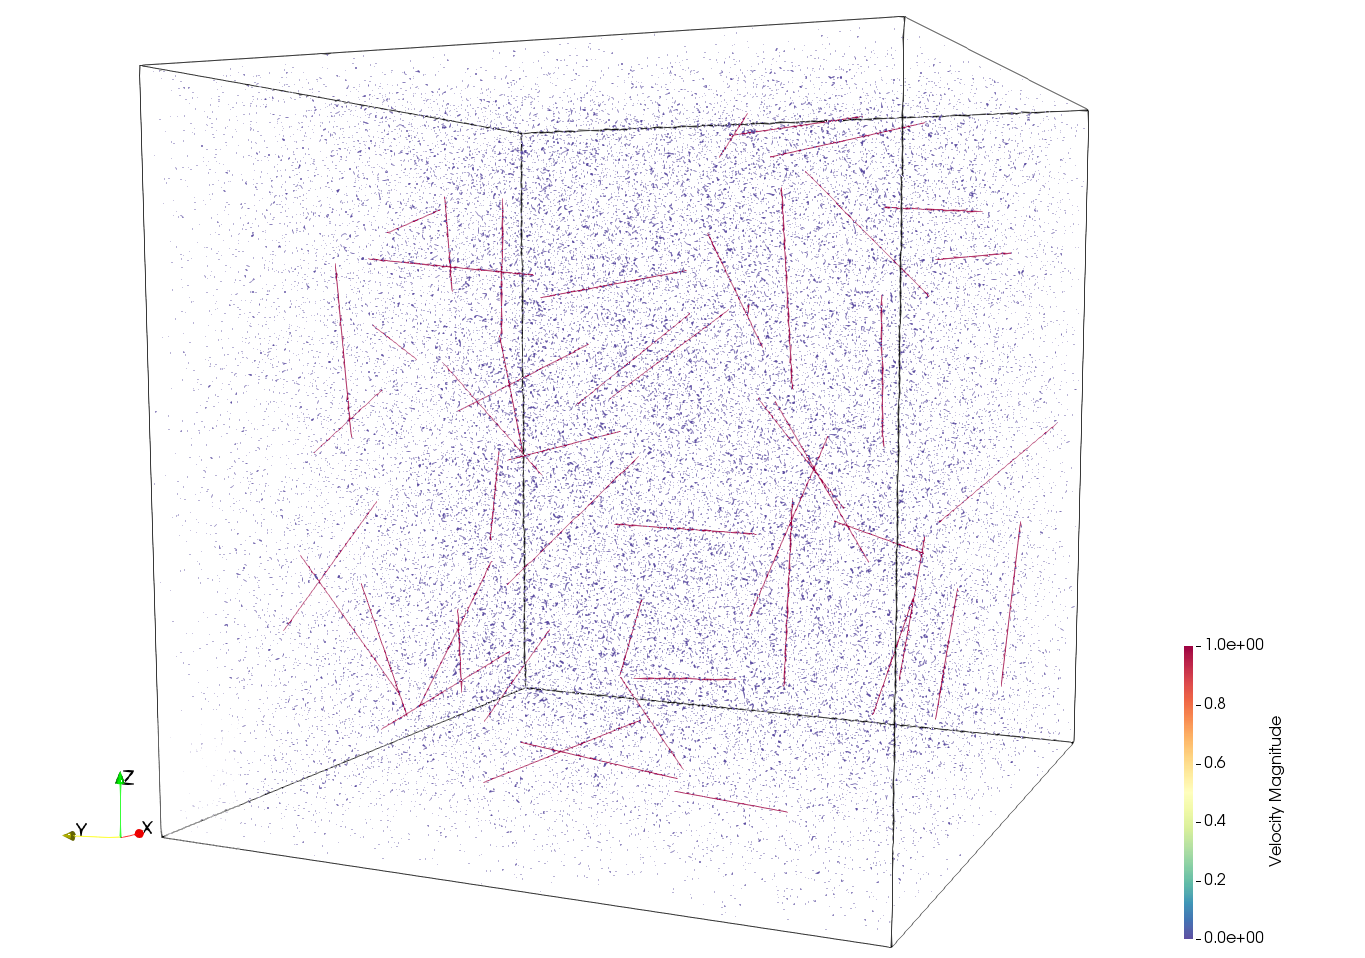
\includegraphics[width=\textwidth]{img/benchmark_example}
	\caption{Visualisation du cas test.}
	\label{fig:benchmark_exemple}
\end{figure}

\subsubsection{Résultats}

\paragraph{Temps d'exécution}
Les différents algorithmes ont été exécutés sur le cas test précédent. Les résultats obtenus sont à relativiser dans la mesure ou le travail d'optimisation n'a pas été le même sur tous les algorithmes. Ils permettent tout de même de comparer les ordres de grandeur des temps d'exécution. Le tableau \ref{tab:bench_temps_algos} recense les temps mesurés pour les différents algorithmes. Pour l'algorithme de fusion de proximité, la détection représente la somme des temps pour toutes les détections de sous-pas de temps, alors que pour les autres algorithmes seule la détection initiale est prise en compte.

\begin{table}[H]
	\centering
	\begin{tabulary}{\textwidth}{l|CC}
		\textbf{Algorithme} & \textbf{Temps détection (ms)} & \textbf{Temps Gestion (ms)} \\
		Fusion de Proximité (estimé) & > 56 000  & 0 \\
		Dynamique séquentiel  & 2 800 & 30 \\
		Dynamique Parallèle & 2 800 & 30 \\
	\end{tabulary}	
	\caption{Mesures de temps d'exécution.}
	\label{tab:bench_temps_algos}
\end{table}

Le découpage par grille dans l'algorithme de Fusion de Proximité n'a pas été implémenté, donc les résultats de la mesure ne sont pas représentatifs de la réalité de la performance de cet algorithme ( $ > 300s$ ). Cependant, il est possible d'estimer le temps d'exécution. L'algorithme doit effectuer des pas de temps $dt_{col} = \frac{r_{col}}{2v_{max}} = 0.025$ soit 40 pas de temps. En estimant la détection statique deux fois plus rapide que la détection dynamique, l'algorithme devrait passer au moins 20 fois plus de temps dans la phase détection que les algorithmes dynamiques.

Les deux algorithmes dynamiques se comportent de la même manière : le temps de calcul est dépensé principalement lors de la phase de détection. L'algorithme de gestion de collisions influe peu sur la performance globale, et l'algorithme le plus simple (séquentiel) peut être utilisé.

\paragraph{Nombre de tests}

Pour les algorithmes dynamiques, les optimisations utilisées réduisent significativement le nombre de tests de collision à effectuer. Le tableau \ref{tab:nb_collision_test} donne le nombre d'opérations effectué pour l'exécution des algorithmes dynamiques sur le cas test précédent. 

\begin{table}[H]
	\centering
	\begin{tabulary}{\textwidth}{C|CCCC}
		\textbf{$N$} 		& \textbf{$N^2$} 		& \textbf{Tests Sphères} & \textbf{Tests exacts} & \textbf{Collisions détectées} \\
		\hline
		$6.5 \cdot 10^{5}$ 	& $4.2 \cdot 10^{11}$ 	& $8.1 \cdot 10^{7}$ 	 & 231					& 2 \\
	\end{tabulary}	
	\caption{Nombre d'opérations effectuées.}
	\label{tab:nb_collision_test}
\end{table}

On remarque que le nombre de tests entre sphères correspond bien à la formule \ref{for:complexite_detection_grille}. L'espace est découpé en 64 boites dans chaque dimension. En appliquant la formule, on obtient $D_B\approx2.5$ et donc $C_\text{detection} \approx  10^{8}$. Le taux de faux-positifs est très faible pour l'utilisation des sphères englobantes. Seul un très faible nombre de tests exacts doivent être exécutés. 

Le nombre de collisions qui ont lieu au cours du pas de temps est très faible, même lorsque l'on double le nombre de boucles et que l'on augmente la vitesse de déplacement des lignes.

\paragraph{Parallélisme}

L'algorithme de détection dynamique des collisions peut être parallélisé en utilisant OpenMP/MPI comme décrit dans la partie \ref{sec:parallelisation_detection}. La scalabilité OpenMP a été testée et la figure \ref{fig:speedup_detection} illustre les résultats. La performance de l'algorithme (en itérations par seconde) a été mesurée fonction du nombre de threads utilisés.

\begin{figure}[H]
	\centering
	\includetikz{img/speedup_detection}
	%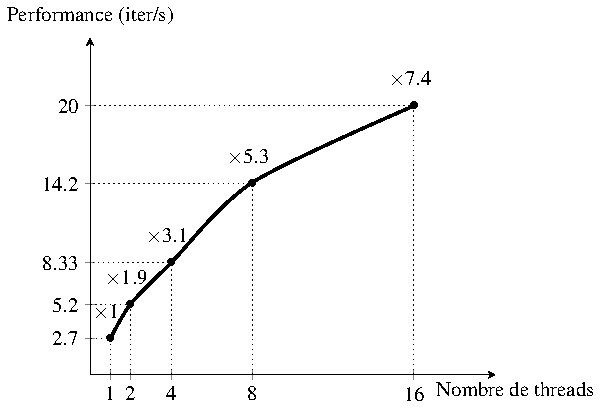
\includegraphics[height=0.4\textheight]{img/speedup_detection}
	\caption{Scalabilité de l'algorithme de détection}
	\label{fig:speedup_detection}
\end{figure}

La construction de la grille uniforme n'est pas prise en compte ici, mais peut représenter une portion importante du temps de calcul car elle se parallélise moins bien. Il faut trouver un compromis quand à la taille de boites de la grille uniforme. Une grille trop grande augmente la complexité de la détection, mais des boites trop petites augmentent le temps de construction de la grille.


\subsection*{Conclusion}

Dans cette section, nous avons étudié plusieurs algorithmes de gestion des collisions pour la formation de jonction pour la dynamique des dislocations. Nous avons décrit comment implémenter de manière sûre et efficace les algorithmes de détection et de gestion des collision. Après l'étude de ces différents algorithmes, notre choix s'est porté sur l'algorithme de gestion des collisions dynamique séquentiel avec re-calcul et sans déplacement. 

\paragraph{}
L'algorithme de gestion des collisions dynamique séquentiel avec re-calcul et sans déplacement de collisions a été intégré dans OptiDis. D'autres travaux liés au parallélisme MPI doivent être menés avant de pouvoir mesurer précisément la performance de l'algorithme de collision au sein du logiciel de simulation.

\end{document}